\section{Eulerkredse}

En bestemt type af kredse gennemgår alle kanter i en graf og kaldes Eulerkredse. 

\begin{defn}\label{euler_def}
En Eulerkreds er en simpel kreds i grafen $G$ som indeholder hver kant i $G$.
En Eulervej er en simpel vej i grafen $G$, som indeholder hver kant i $G$.  
\end{defn}
\noindent Eksempler på en Eulerkreds og en Eulervejkan ses her: \\
\begin{figure}[h]
\centering
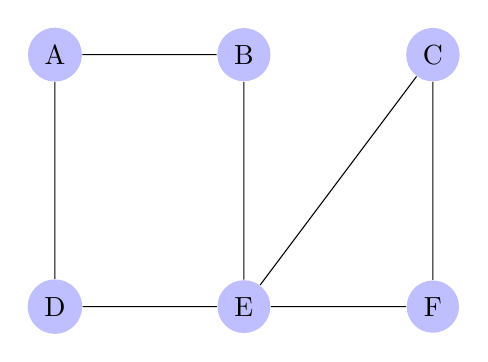
\begin{tikzpicture}
[scale=.8,auto=left,every node/.style={circle,fill=blue!25}]
  \node (n6) at (3,2) {D};
  \node (n4) at (3,6) {A};
  \node (n5) at (6,2) {E};
  \node (n1) at (6,6) {B};
  \node (n2) at (9,2) {F};
  \node (n3) at (9,6) {C};
  \foreach \from/\to in {n6/n4,n5/n1,n2/n5,n2/n3,n1/n4,n6/n5,n5/n3}
    \draw (\from) -- (\to);
\end{tikzpicture}
\caption{Euler kreds} 
\label{euler_kreds}
\end{figure}

\noindent Et eksempel på en Eulerkreds i Figur \ref{euler_kreds} kan være: $A,B,E,C,F,E,D,A$

\begin{figure}[h]
\centering
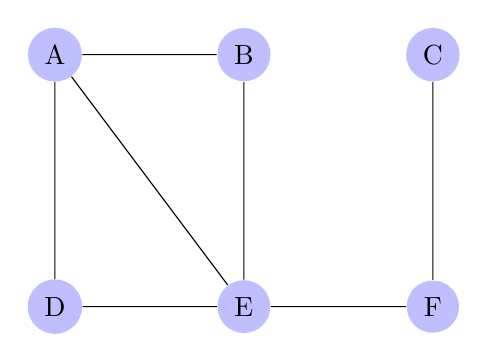
\begin{tikzpicture}
[scale=.8,auto=left,every node/.style={circle,fill=blue!25}]
  \node (n6) at (3,2) {D};
  \node (n4) at (3,6) {A};
  \node (n5) at (6,2) {E};
  \node (n1) at (6,6) {B};
  \node (n2) at (9,2) {F};
  \node (n3) at (9,6) {C};
  \foreach \from/\to in {n6/n4,n5/n1,n2/n5,n2/n3,n1/n4,n6/n5,n4/n5}
    \draw (\from) -- (\to);
\end{tikzpicture}
\caption{Euler vej} 
\label{euler_vej}
\end{figure}

\noindent Et eksempel på en Eulervej i Figur \ref{euler_vej} kan være: $A,B,E,D,A,E,F,C$

Der eksiserer ikke en Eulerkreds i alle grafer. 
For at der kan eksiserer en eulerkreds i en sammenhægende multigraf skal Sætning \ref{Eulerkreds_multigraf} gælde. 

\begin{thm}\label{Eulerkreds_multigraf}
En sammenhængende multigraf med mindst 2 knuder, har en Eulerkreds hvis og kun hvis, hver knude er af lige grad.
\end{thm}

\begin{proof} 
En kreds begynder i en knude $a$ og fortsætter langs en kant, som en incident med $a$, til en nu knude $b$. 
Denne kant kaldes $(a,b)$, kanten bidrager med 1 til $deg(a)$. 
Hver gang kredsen passere gennem en knude, tilføjes 2 til graden af denne knude. 
Til sidst ender kredsen tilbage i $a$, og bidrager igen med 1 til $deg(a)$. 
Derfor må $deg(a)$ være lige og graden af hver knude må også være lige.  
\end{proof} 

\noindent Det er muligt at lave en algoritme som kan finde en Eulerkreds i en multigraf.

En sådanne algoritme vil første tage udgangspunkt i en tilfældig delkreds i graf G. 
Hvorefter der indeførers en variabel H, som som en lig med G, foruden kanterne i den tilfældige delkreds. 
Så længe H indeholder kanter, vil en løkke køre. 
Under denne løkke dannes en ny delkreds i H, hvor en af knuderne skal også være endepunkt for en kant i en tidligere delkreds.
Dernæst fjerens kanterne i delkredsen fra H, sammen med enventuelt isolerede knuder. 
Til sidst sammensættes delkredsene til en kreds og denne kreds retuneres.
Dette kan ses i Algoritme \ref{algoritme_euler}.
Der findes også andre algoritmer som kan finde Eulerkredse i en graf, men disse bliver ikke nævnt i dette projekt.\\
  

\begin{algorithm}
\caption{Eulerkredse}
\label{algoritme_euler}
\textbf{procedure} Euler(G: sammenhængende mulitgraf med knuder af lige grad)\\
$kreds:=$ en kreds i G begynder i en vilkårlig knude, med kanter der danner en kreds, som retunerer til startknuden.\\
$H:= G$ med kanterne fra $kreds$ fjernet\\
\textbf{når} $H$ har kanter\\
$\-$ $\-$ $\-$ $\-$ $\-$ $\-$
$delkreds:=$ en kreds i $H$ der begynder i en knude i $H$ som også er et endepunkt af en kant i $kreds$ \\ 
$\-$ $\-$ $\-$ $\-$ $\-$ $\-$
$H:=$ $H$ uden kanterne af delkredsen samt alle isolerede knuder fjernet \\
$\-$ $\-$ $\-$ $\-$ $\-$ $\-$
$kreds:=$ $kreds$ med $delkreds$ indsat ved den passende knude \\ 
\textbf{retuner} $kreds$ ($kreds$ er en Eulerkreds)
\end{algorithm}

$\-$ $\-$ $\-$ $\-$ $\-$ $\-$ \\
\noindent Hvis der ikke findes en Eulerkreds i en graf, kan der godt eksistere en Eulervej. 
For at der kan findes en Eulervej skal Sætning \ref{Eulervej_multigraf} gælde. 

\begin{thm} \label{Eulervej_multigraf}
En sammenhængende multigraf graf G har en Eulervej, men ikke en Eulerkreds, hvis og kun hvis den har præcist to knuder er ulige grad.  
\end{thm} 

\begin{proof}
Antag at en sammenhængende multigraf G har en Eulervej fra $a$ til $b$, men ikke en Eulerkreds. 
Den første kant som passeres på vejen bidrager med 1 til $deg(a)$. 
Hver gang vejen passerer knuden $a$ vil 2 tilføjes til $deg(a)$. 
Den sidste kant på vejen bidrager 1 til graden af endepunktet for vejen, $deg(b)$. 
Ligesom for $a$, kan vejen krydse $b$. 
Hver gange dette måtte ske tilføjes 2 til graden af $b$. 
Dette ender ud i at $a$ og $b$ altid vil være af ulige grad. 
Alle andre knuder på vejen vil være af lige grad, fordi at 2 tilføjes til graden af en knude, hver gang en knude passeres.  
\end{proof}

